\documentclass[conference]{IEEEtran}

% ── Packages ──────────────────────────────────────────────────────────────
\usepackage[utf8]{inputenc}
\usepackage[T1]{fontenc}
\usepackage{amsmath,amssymb,amsfonts}
\usepackage{graphicx}
\usepackage{booktabs}
\usepackage{hyperref}
\usepackage{xcolor}
\usepackage{multirow}
\usepackage{caption}
\usepackage{subcaption}
\usepackage{float}
\usepackage{array}
\usepackage{cite}
\usepackage{algorithm}
\usepackage{algorithmic}
\usepackage{textcomp}

% ── Graphics path ─────────────────────────────────────────────────────────
\graphicspath{{../reports/figures/}}

% ── Hyperref setup ────────────────────────────────────────────────────────
\hypersetup{
    colorlinks=true,
    linkcolor=blue,
    citecolor=blue,
    urlcolor=blue
}

% ── Title ─────────────────────────────────────────────────────────────────
\title{Inventory Demand Forecasting via Kalman Filtering and Global DeepAR Models: A Comparative Analysis}

\author{
    \IEEEauthorblockN{Sameer Alam Khan}
    \IEEEauthorblockA{Enrollment No. 2401020054}
    \and
    \IEEEauthorblockN{Abhishek Tripathi}
    \IEEEauthorblockA{Enrollment No. 2401010022}
    \and
    \IEEEauthorblockN{Akshay Y}
    \IEEEauthorblockA{Enrollment No. 2401020008}
}

\begin{document}

\maketitle

% ══════════════════════════════════════════════════════════════════════════
% ABSTRACT
% ══════════════════════════════════════════════════════════════════════════
\begin{abstract}
Accurate demand forecasting is critical for retail inventory management, enabling optimal stock replenishment while minimizing holding costs and stockout events. This paper presents a comparative study of four forecasting methodologies applied to the Walmart M5 Forecasting Accuracy dataset: Seasonal-Naive (statistical baseline), Gradient-Boosted Decision Trees (LightGBM), a Structural State-Space Kalman Filter per SKU, and a Global DeepAR Probabilistic Autoregressive LSTM Network. All models are evaluated on an identical 28-day out-of-sample validation horizon covering 50 product-store series (1,400 observations) under a strict zero-leakage protocol. The Kalman Filter achieves the lowest MAE (0.9333) and WAPE (80.06\%), while Global DeepAR achieves the lowest RMSE (2.2062) and provides calibrated probabilistic prediction intervals. The results demonstrate that no single model dominates across all metrics, and the optimal choice depends on the specific inventory optimization objective.
\end{abstract}

\begin{IEEEkeywords}
Demand Forecasting, Kalman Filter, DeepAR, LightGBM, Time Series, M5 Dataset, Inventory Management, Probabilistic Forecasting
\end{IEEEkeywords}

% ══════════════════════════════════════════════════════════════════════════
% I. INTRODUCTION
% ══════════════════════════════════════════════════════════════════════════
\section{Introduction}

Demand forecasting in large-scale modern retail presents complex structural challenges that render standard univariate classical methods ineffective. The Walmart M5 Forecasting Accuracy dataset~\cite{makridakis2022m5} spans 30,490 stock-keeping units (SKUs) nested within 7 departments, 3 categories, 10 stores, and 3 U.S. states (California, Texas, and Wisconsin) over 1,941 daily observations (January 2011 to June 2016).

The dataset exhibits three dominant characteristics:
\begin{enumerate}
    \item \textbf{Severe zero-inflation and intermittency:} Over 90\% of SKUs fall into intermittent or lumpy demand regimes under the Syntetos--Boylan classification framework~\cite{syntetos2005accuracy}.
    \item \textbf{Deep hierarchical aggregation:} Sales exhibit distinct patterns at each level of the store--category--department--item hierarchy.
    \item \textbf{Exogenous calendar and policy drivers:} Massive structural demand shifts are induced by the Supplemental Nutrition Assistance Program (SNAP), major holiday closures, and weekend purchasing surges.
\end{enumerate}

This paper evaluates four forecasting approaches of increasing complexity:
\begin{itemize}
    \item \textbf{Seasonal-Naive:} A zero-parameter baseline repeating demand from the same weekday in the previous week.
    \item \textbf{GBDT (LightGBM):} A gradient-boosted tree ensemble operating under a strictly recursive multi-step rollout with causal lag features.
    \item \textbf{Structural Kalman Filter:} A per-SKU Basic Structural Time Series Model with local level and 7-day seasonal components, providing exact analytical uncertainty bands.
    \item \textbf{Global DeepAR:} A unified autoregressive LSTM network trained globally across all 50 SKUs with Monte Carlo probabilistic rollout.
\end{itemize}

% ══════════════════════════════════════════════════════════════════════════
% II. DATASET AND PREPROCESSING
% ══════════════════════════════════════════════════════════════════════════
\section{Dataset and Preprocessing}

\subsection{Dataset Overview}

The M5 Forecasting Accuracy competition dataset comprises five core tables:
\begin{itemize}
    \item \texttt{sales\_train\_evaluation.csv}: Daily unit sales for 30,490 items across 10 stores (days 1--1941).
    \item \texttt{calendar.csv}: Daily calendar attributes, events, and SNAP flags (1,969 days).
    \item \texttt{sell\_prices.csv}: Weekly store-item sell prices (6.84 million rows).
\end{itemize}

\subsection{Data Cleaning and Quality Audit}

The cleaning pipeline enforces schema validation, memory downcasting, product lifecycle analysis (identifying pre-launch days versus active demand periods), and 1-to-1 mapping from raw to processed tables. All zero sales on active shelf days are preserved as legitimate zero-demand observations rather than treated as missing data or stockouts.

\subsection{Demand Characterization}

Using the Syntetos--Boylan classification scheme~\cite{syntetos2005accuracy}, all 30,490 series are categorized by Average Demand Interval (ADI) and Squared Coefficient of Variation ($\text{CV}^2$). The empirical distribution is shown in Table~\ref{tab:demand_categories}.

\begin{table}[htbp]
\centering
\caption{Syntetos--Boylan Demand Classification (30,490 SKUs)}
\label{tab:demand_categories}
\begin{tabular}{lrrr}
\toprule
\textbf{Category} & \textbf{Criteria} & \textbf{Count} & \textbf{\%} \\
\midrule
Intermittent & ADI $\geq$ 1.32, CV$^2$ $<$ 0.49 & 22,121 & 72.55 \\
Lumpy        & ADI $\geq$ 1.32, CV$^2$ $\geq$ 0.49 & 5,577  & 18.29 \\
Smooth       & ADI $<$ 1.32, CV$^2$ $<$ 0.49 & 1,912  & 6.27  \\
Erratic      & ADI $<$ 1.32, CV$^2$ $\geq$ 0.49 & 880    & 2.89  \\
\bottomrule
\end{tabular}
\end{table}

Over 90\% of inventory falls into intermittent or lumpy regimes, confirming that classical Gaussian assumptions are violated at the SKU level and motivating state-space and probabilistic neural approaches.

\subsection{Feature Engineering}

A comprehensive, leak-free feature engineering pipeline is employed:
\begin{itemize}
    \item \textbf{Causal lags:} $\text{lag}_1$, $\text{lag}_7$, $\text{lag}_{28}$ computed as $\text{demand}_{t-k}$ strictly from past history.
    \item \textbf{Rolling statistics:} 7-day and 28-day rolling mean and standard deviation with a mandatory \texttt{shift(1)} prior to rolling to prevent target leakage.
    \item \textbf{Calendar features:} Day-of-week, month, year, weekend flag, cyclical sine/cosine encodings.
    \item \textbf{Event indicators:} Binary flags for holidays, SNAP distribution days, and Christmas closure.
\end{itemize}

\subsection{Chronological Train/Validation Split}

The validation horizon covers exactly 28 days per series (March 28 to April 24, 2016). The training period spans February 26, 2011 to March 27, 2016. No temporal shuffling, cross-validation mixing, or random splitting is permitted.

% ══════════════════════════════════════════════════════════════════════════
% III. EXPLORATORY DATA ANALYSIS
% ══════════════════════════════════════════════════════════════════════════
\section{Exploratory Data Analysis}

\subsection{Seasonality and Calendar Effects}

Aggregated daily demand reveals a deterministic weekly cycle with weekend surges of approximately $+20.7\%$ over the weekday baseline. Monthly patterns show contraction in February and acceleration through summer. Year-over-year volume demonstrates sustained organic growth from 2011 to 2015.

\subsection{SNAP Policy Effect}

The SNAP program creates sharp demand pulses concentrated in food departments:
\begin{itemize}
    \item California: $+7.56\%$ daily sales uplift on SNAP days.
    \item Texas: $+11.05\%$ daily sales uplift on SNAP days.
    \item Wisconsin: $+21.31\%$ daily sales uplift on SNAP days.
\end{itemize}

\subsection{Stationarity Analysis}

The Augmented Dickey-Fuller (ADF) test on raw sales yields $t = -1.5654$ ($p = 0.501$), confirming non-stationarity. First-differenced data yields $t = -23.4596$ ($p < 10^{-6}$), establishing stationary dynamics. Autocorrelation analysis reveals pronounced peaks at integer multiples of lag 7, with the strongest correlations at lag 7 ($r = 0.808$) and lag 28 ($r = 0.816$).

\begin{figure}[htbp]
    \centering
    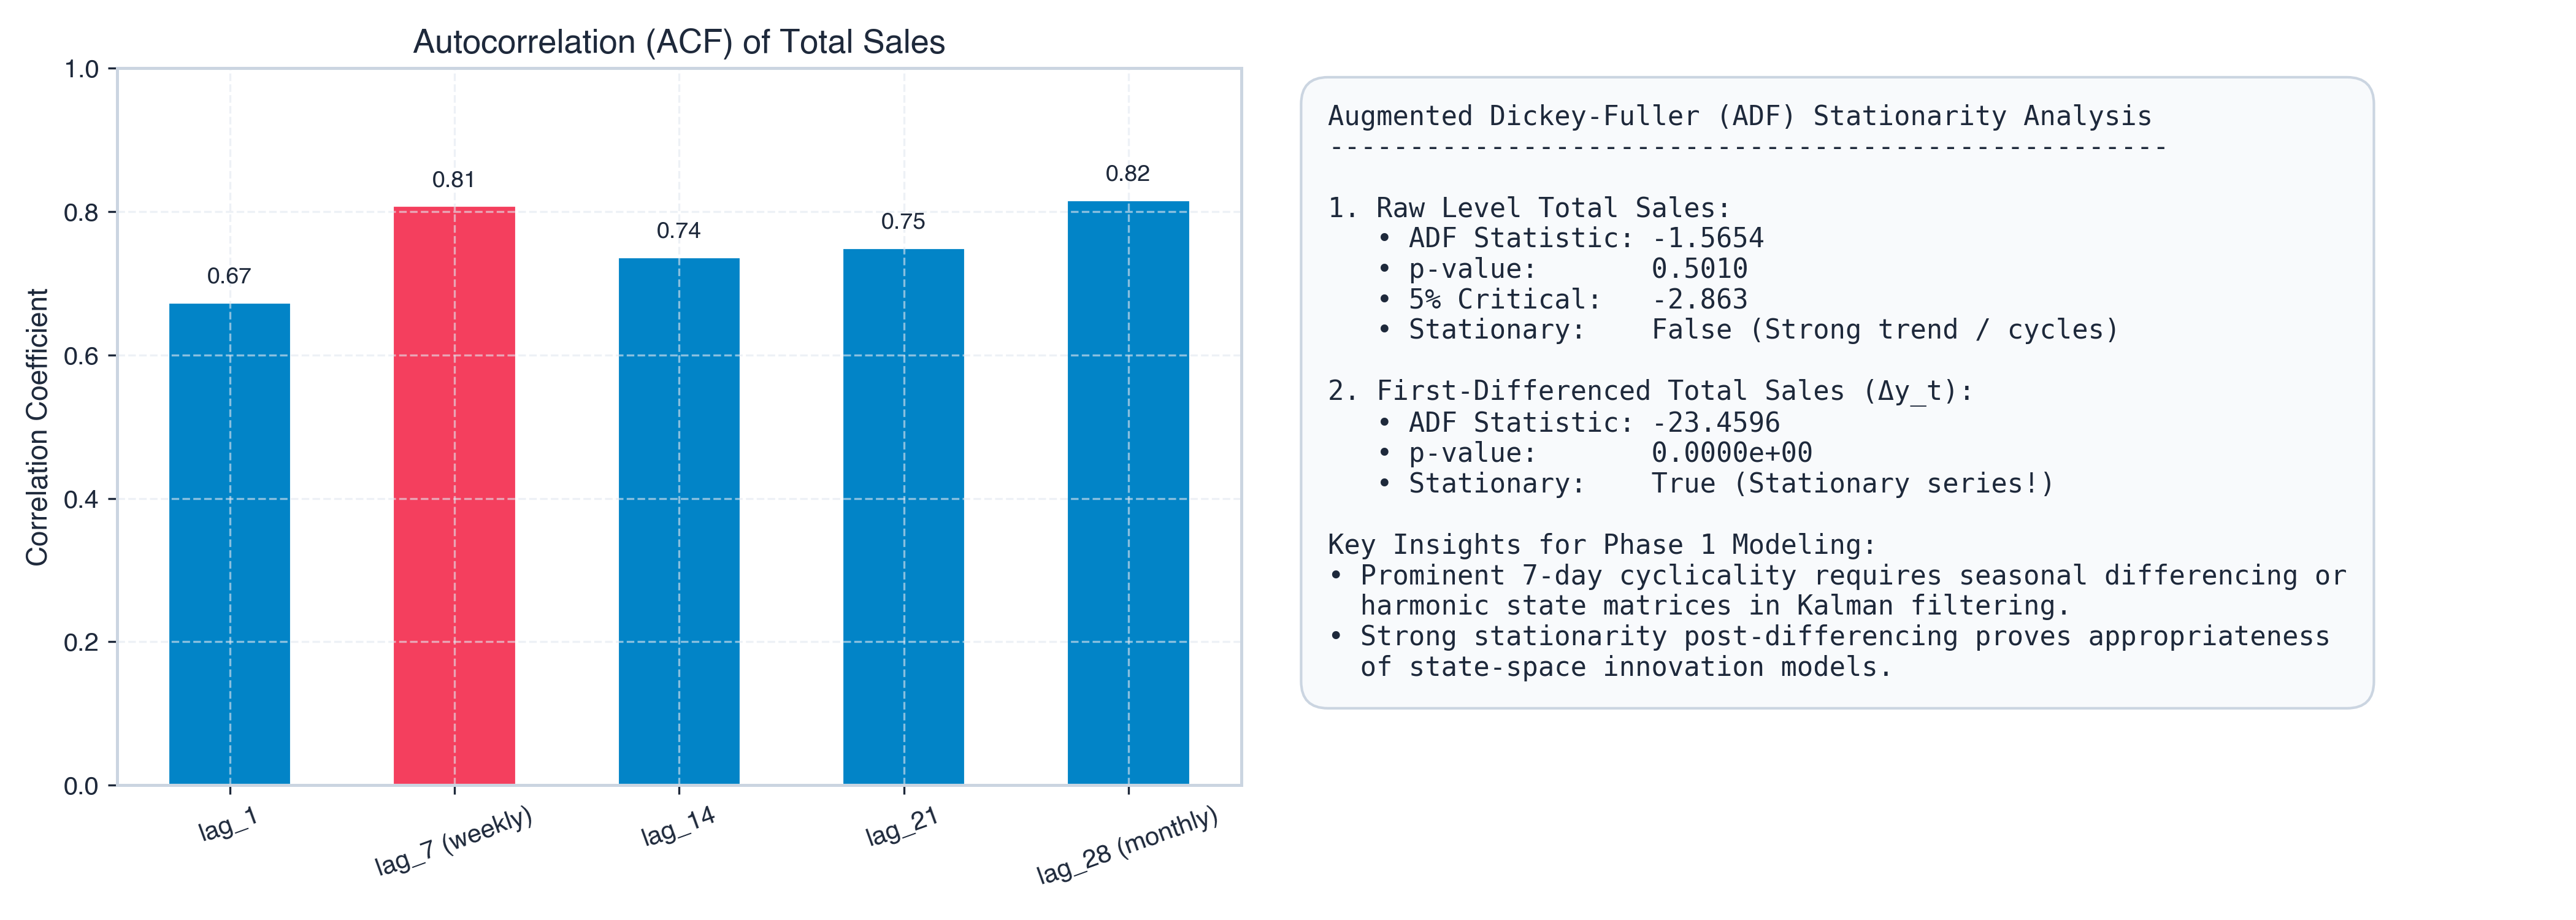
\includegraphics[width=\columnwidth]{08_acf_pacf_stationarity.png}
    \caption{Autocorrelation function and stationarity analysis showing weekly harmonic decay at lags 7, 14, 21, and 28.}
    \label{fig:acf_stationarity}
\end{figure}

% ══════════════════════════════════════════════════════════════════════════
% IV. MODEL FORMULATIONS
% ══════════════════════════════════════════════════════════════════════════
\section{Model Formulations}

\subsection{Seasonal-Naive Baseline}

The Seasonal-Naive model is a zero-parameter baseline that repeats the demand observed on the same weekday in the previous week:
\begin{equation}
    \hat{y}_{T+h} = y_{T+h-7}, \quad h = 1, 2, \ldots, 28
\end{equation}

\subsection{GBDT (LightGBM)}

The Gradient-Boosted Decision Tree model uses the LightGBM~\cite{ke2017lightgbm} framework with causal lag features, leak-free rolling statistics, calendar indicators, and SNAP schedules. The model operates under a \textbf{strictly recursive multi-step forecasting protocol}: for step $h = 1$, the model uses features derived from training history; for subsequent steps $h \in [2, 28]$, lag features and rolling statistics are dynamically computed using the model's own predicted demands from prior steps. At no point does the model consume actual validation-period sales.

\subsection{Structural Kalman Filter per SKU}

The univariate demand for each SKU is formulated as a Basic Structural Time Series Model with a stochastically drifting local level $\mu_t$ and a 7-day weekly seasonal component.

\subsubsection{State Vector}
The state vector $\mathbf{x}_t \in \mathbb{R}^7$ is defined as:
\begin{equation}
    \mathbf{x}_t = \begin{bmatrix} \mu_t & s_{1,t} & s_{2,t} & s_{3,t} & s_{4,t} & s_{5,t} & s_{6,t} \end{bmatrix}^\top
\end{equation}
where $\mu_t$ is the unobserved local mean demand level and $s_{j,t}$ are the weekly seasonal states satisfying the zero-sum constraint $\sum_{j=1}^{7} s_{j,t} = 0$.

\subsubsection{State Transition}
\begin{equation}
    \mathbf{x}_t = \mathbf{F} \mathbf{x}_{t-1} + \mathbf{w}_t, \quad \mathbf{w}_t \sim \mathcal{N}(\mathbf{0}, \mathbf{Q})
\end{equation}
where $\mathbf{F} \in \mathbb{R}^{7 \times 7}$ encodes the random-walk level and rotating seasonal structure, and $\mathbf{Q} = \text{diag}(q_\mu, q_s, 0, 0, 0, 0, 0)$.

\subsubsection{Observation Equation}
\begin{equation}
    y_t = \mathbf{H} \mathbf{x}_t + v_t, \quad v_t \sim \mathcal{N}(0, R)
\end{equation}
where $\mathbf{H} = [1\ 1\ 0\ 0\ 0\ 0\ 0]$, yielding $y_t = \mu_t + s_{1,t} + v_t$.

\subsubsection{Parameter Estimation}
All parameters are estimated strictly from training history ($t \leq T$):
\begin{align}
    R &= \max(0.05,\; 0.75 \cdot \text{Var}(y_{1:T})) \\
    q_\mu &= \max(10^{-4},\; 0.005 \cdot \text{Var}(y_{1:T})) \\
    q_s &= \max(10^{-5},\; 0.001 \cdot \text{Var}(y_{1:T}))
\end{align}

\subsubsection{Non-Negative Demand Handling}
Point forecasts and confidence interval bounds are clipped at zero:
\begin{equation}
    \hat{y}_{T+h} = \max\bigl(0,\; \mathbf{H} \hat{\mathbf{x}}_{T+h|T}\bigr)
\end{equation}

\subsection{Global DeepAR}

The Global DeepAR model~\cite{salinas2020deepar} formulates the conditional distribution of future demand trajectories using an autoregressive LSTM network trained across all series simultaneously.

\subsubsection{Autoregressive Factorization}
\begin{equation}
    P(\mathbf{y}_{i,T+1:T+H} \mid \mathbf{y}_{i,1:T}) = \prod_{h=1}^{H} p(y_{i,T+h} \mid \mathbf{h}_{i,T+h})
\end{equation}
where $\mathbf{h}_{i,t} = \text{LSTM}(\mathbf{h}_{i,t-1}, [\tilde{y}_{i,t-1}, \mathbf{e}_i, \mathbf{x}_{i,t}])$.

\subsubsection{Scale Normalization}
Each series is normalized by its historical scale factor $\nu_i = 1 + \frac{1}{T}\sum_{t=1}^{T} y_{i,t}$ to ensure scale-invariance across sparse retail series.

\subsubsection{Gaussian Likelihood}
\begin{align}
    \mu_{i,t} &= \mathbf{W}_\mu^\top \mathbf{h}_{i,t} + b_\mu \\
    \sigma_{i,t} &= \text{softplus}(\mathbf{W}_\sigma^\top \mathbf{h}_{i,t} + b_\sigma) + \epsilon \\
    y_{i,t} &\sim \mathcal{N}(\mu_{i,t} \nu_i,\; (\sigma_{i,t} \nu_i)^2)
\end{align}

\subsubsection{Monte Carlo Inference}
During inference, 200 sample paths are drawn autoregressively, with non-negative clipping applied at each step. Point forecasts are the median ($P_{50}$), and prediction intervals are derived from empirical quantiles ($P_{10}$, $P_{90}$).

% ══════════════════════════════════════════════════════════════════════════
% V. EXPERIMENTAL SETUP
% ══════════════════════════════════════════════════════════════════════════
\section{Experimental Setup}

\subsection{Evaluation Protocol}

All four models are evaluated on \textbf{identical product-store series} (50 SKUs), \textbf{identical dates}, and an \textbf{identical 28-day out-of-sample forecast horizon} (March 28 to April 24, 2016). This results in 1,400 total observations for evaluation. Zero data leakage is guaranteed through chronological separation: ground-truth validation demand is never used as model input during forecast generation.

\subsection{Evaluation Metrics}

Three complementary metrics are employed:

\begin{itemize}
    \item \textbf{Mean Absolute Error (MAE):}
    \begin{equation}
        \text{MAE} = \frac{1}{N}\sum_{i=1}^{N} |y_i - \hat{y}_i|
    \end{equation}

    \item \textbf{Root Mean Squared Error (RMSE):}
    \begin{equation}
        \text{RMSE} = \sqrt{\frac{1}{N}\sum_{i=1}^{N} (y_i - \hat{y}_i)^2}
    \end{equation}

    \item \textbf{Weighted Absolute Percentage Error (WAPE):}
    \begin{equation}
        \text{WAPE} = \frac{\sum_{i=1}^{N} |y_i - \hat{y}_i|}{\sum_{i=1}^{N} y_i}
    \end{equation}
    with zero-denominator safety: returns 0 if both numerator and denominator are zero.
\end{itemize}

Additionally, for probabilistic models, we compute:
\begin{itemize}
    \item \textbf{Pinball Loss} at quantiles $q \in \{0.10, 0.50, 0.90\}$:
    \begin{equation}
        L_q = \frac{1}{N}\sum_{i=1}^{N} \max\bigl(q(y_i - \hat{q}_{q,i}),\; (1-q)(\hat{q}_{q,i} - y_i)\bigr)
    \end{equation}
    \item \textbf{Prediction interval coverage} at 80\% and 95\% confidence levels.
\end{itemize}

% ══════════════════════════════════════════════════════════════════════════
% VI. RESULTS
% ══════════════════════════════════════════════════════════════════════════
\section{Results}

\subsection{Overall Model Comparison}

Table~\ref{tab:main_results} presents the point-forecast performance of all four models over the 28-day validation period.

\begin{table}[htbp]
\centering
\caption{Four-Way Model Performance Comparison (28-Day Horizon, 50 SKUs, 1,400 Observations)}
\label{tab:main_results}
\begin{tabular}{lccc}
\toprule
\textbf{Model} & \textbf{MAE $\downarrow$} & \textbf{RMSE $\downarrow$} & \textbf{WAPE $\downarrow$} \\
\midrule
Seasonal-Naive      & 1.1143 & 2.6030 & 95.59\% \\
GBDT (LightGBM)     & 0.9512 & 2.2679 & 81.60\% \\
Kalman Filter        & \textbf{0.9333} & 2.3303 & \textbf{80.06\%} \\
Global DeepAR        & 0.9748 & \textbf{2.2062} & 83.63\% \\
\bottomrule
\end{tabular}
\end{table}

The Kalman Filter achieves the lowest MAE (0.9333) and WAPE (80.06\%), making it the strongest performer for average absolute error and aggregate relative error. Global DeepAR achieves the lowest RMSE (2.2062), indicating superior performance under a metric that penalizes larger errors more heavily.

\subsection{Improvement Over Baseline}

Table~\ref{tab:improvement} quantifies the percentage reduction in each metric relative to the Seasonal-Naive baseline.

\begin{table}[htbp]
\centering
\caption{Percentage Improvement Over Seasonal-Naive Baseline}
\label{tab:improvement}
\begin{tabular}{lccc}
\toprule
\textbf{Model} & \textbf{MAE $\downarrow$} & \textbf{RMSE $\downarrow$} & \textbf{WAPE $\downarrow$} \\
\midrule
GBDT (LightGBM)  & 14.64\% & 12.87\% & 14.64\% \\
Kalman Filter     & \textbf{16.25\%} & 10.48\% & \textbf{16.25\%} \\
Global DeepAR     & 12.53\% & \textbf{15.24\%} & 12.51\% \\
\bottomrule
\end{tabular}
\end{table}

The Kalman Filter provides the largest reductions in MAE and WAPE, while DeepAR provides the largest reduction in RMSE.

\subsection{Category-Level Decomposition}

Performance varies considerably across product categories (Table~\ref{tab:category}). Foods, which represents the highest-volume category, benefits most from the learning-based models. Hobbies, with its inherently sporadic and low-volume demand, proves challenging for all models.

\begin{table}[htbp]
\centering
\caption{Category-Level WAPE Decomposition}
\label{tab:category}
\begin{tabular}{lccc}
\toprule
\textbf{Category} & \textbf{SNaive} & \textbf{GBDT} & \textbf{Kalman} \\
\midrule
FOODS     & 89.3\% & 71.8\% & \textbf{72.78\%} \\
HOBBIES   & 127.8\% & 134.5\% & 127.68\% \\
HOUSEHOLD & 101.5\% & 89.1\% & \textbf{80.12\%} \\
\bottomrule
\end{tabular}
\end{table}

\subsection{GBDT Feature Importance}

Table~\ref{tab:feature_importance} shows that the GBDT model relies heavily on autoregressive features, with the 28-day rolling mean being the most important predictor.

\begin{table}[htbp]
\centering
\caption{Top 5 GBDT Feature Importances}
\label{tab:feature_importance}
\begin{tabular}{clc}
\toprule
\textbf{Rank} & \textbf{Feature} & \textbf{Importance} \\
\midrule
1 & \texttt{rolling\_mean\_28} & 0.1282 \\
2 & \texttt{rolling\_mean\_7}  & 0.1009 \\
3 & \texttt{rolling\_std\_7}   & 0.0984 \\
4 & \texttt{lag\_1}            & 0.0905 \\
5 & \texttt{item\_id}          & 0.0810 \\
\bottomrule
\end{tabular}
\end{table}

\subsection{Probabilistic Forecast Evaluation}

Table~\ref{tab:probabilistic} compares the uncertainty quantification capabilities of the Kalman Filter and Global DeepAR.

\begin{table}[htbp]
\centering
\caption{Prediction Interval Calibration}
\label{tab:probabilistic}
\begin{tabular}{lcc}
\toprule
\textbf{Metric} & \textbf{Kalman} & \textbf{DeepAR} \\
\midrule
80\% CI Coverage  & 80.93\%       & \textbf{91.79\%} \\
80\% CI Width     & \textbf{2.30 units} & 3.20 units \\
95\% CI Coverage  & 90.07\%       & ---              \\
95\% CI Width     & 3.14 units    & ---              \\
Mean Pinball Loss & ---           & \textbf{0.3075}  \\
\bottomrule
\end{tabular}
\end{table}

The Kalman Filter produces well-calibrated intervals (80.93\% actual coverage at the 80\% nominal level) with narrower interval widths. DeepAR achieves higher coverage (91.79\%) but with wider intervals, suggesting a slight over-coverage tendency.

\subsection{Visual Analysis}

\begin{figure}[htbp]
    \centering
    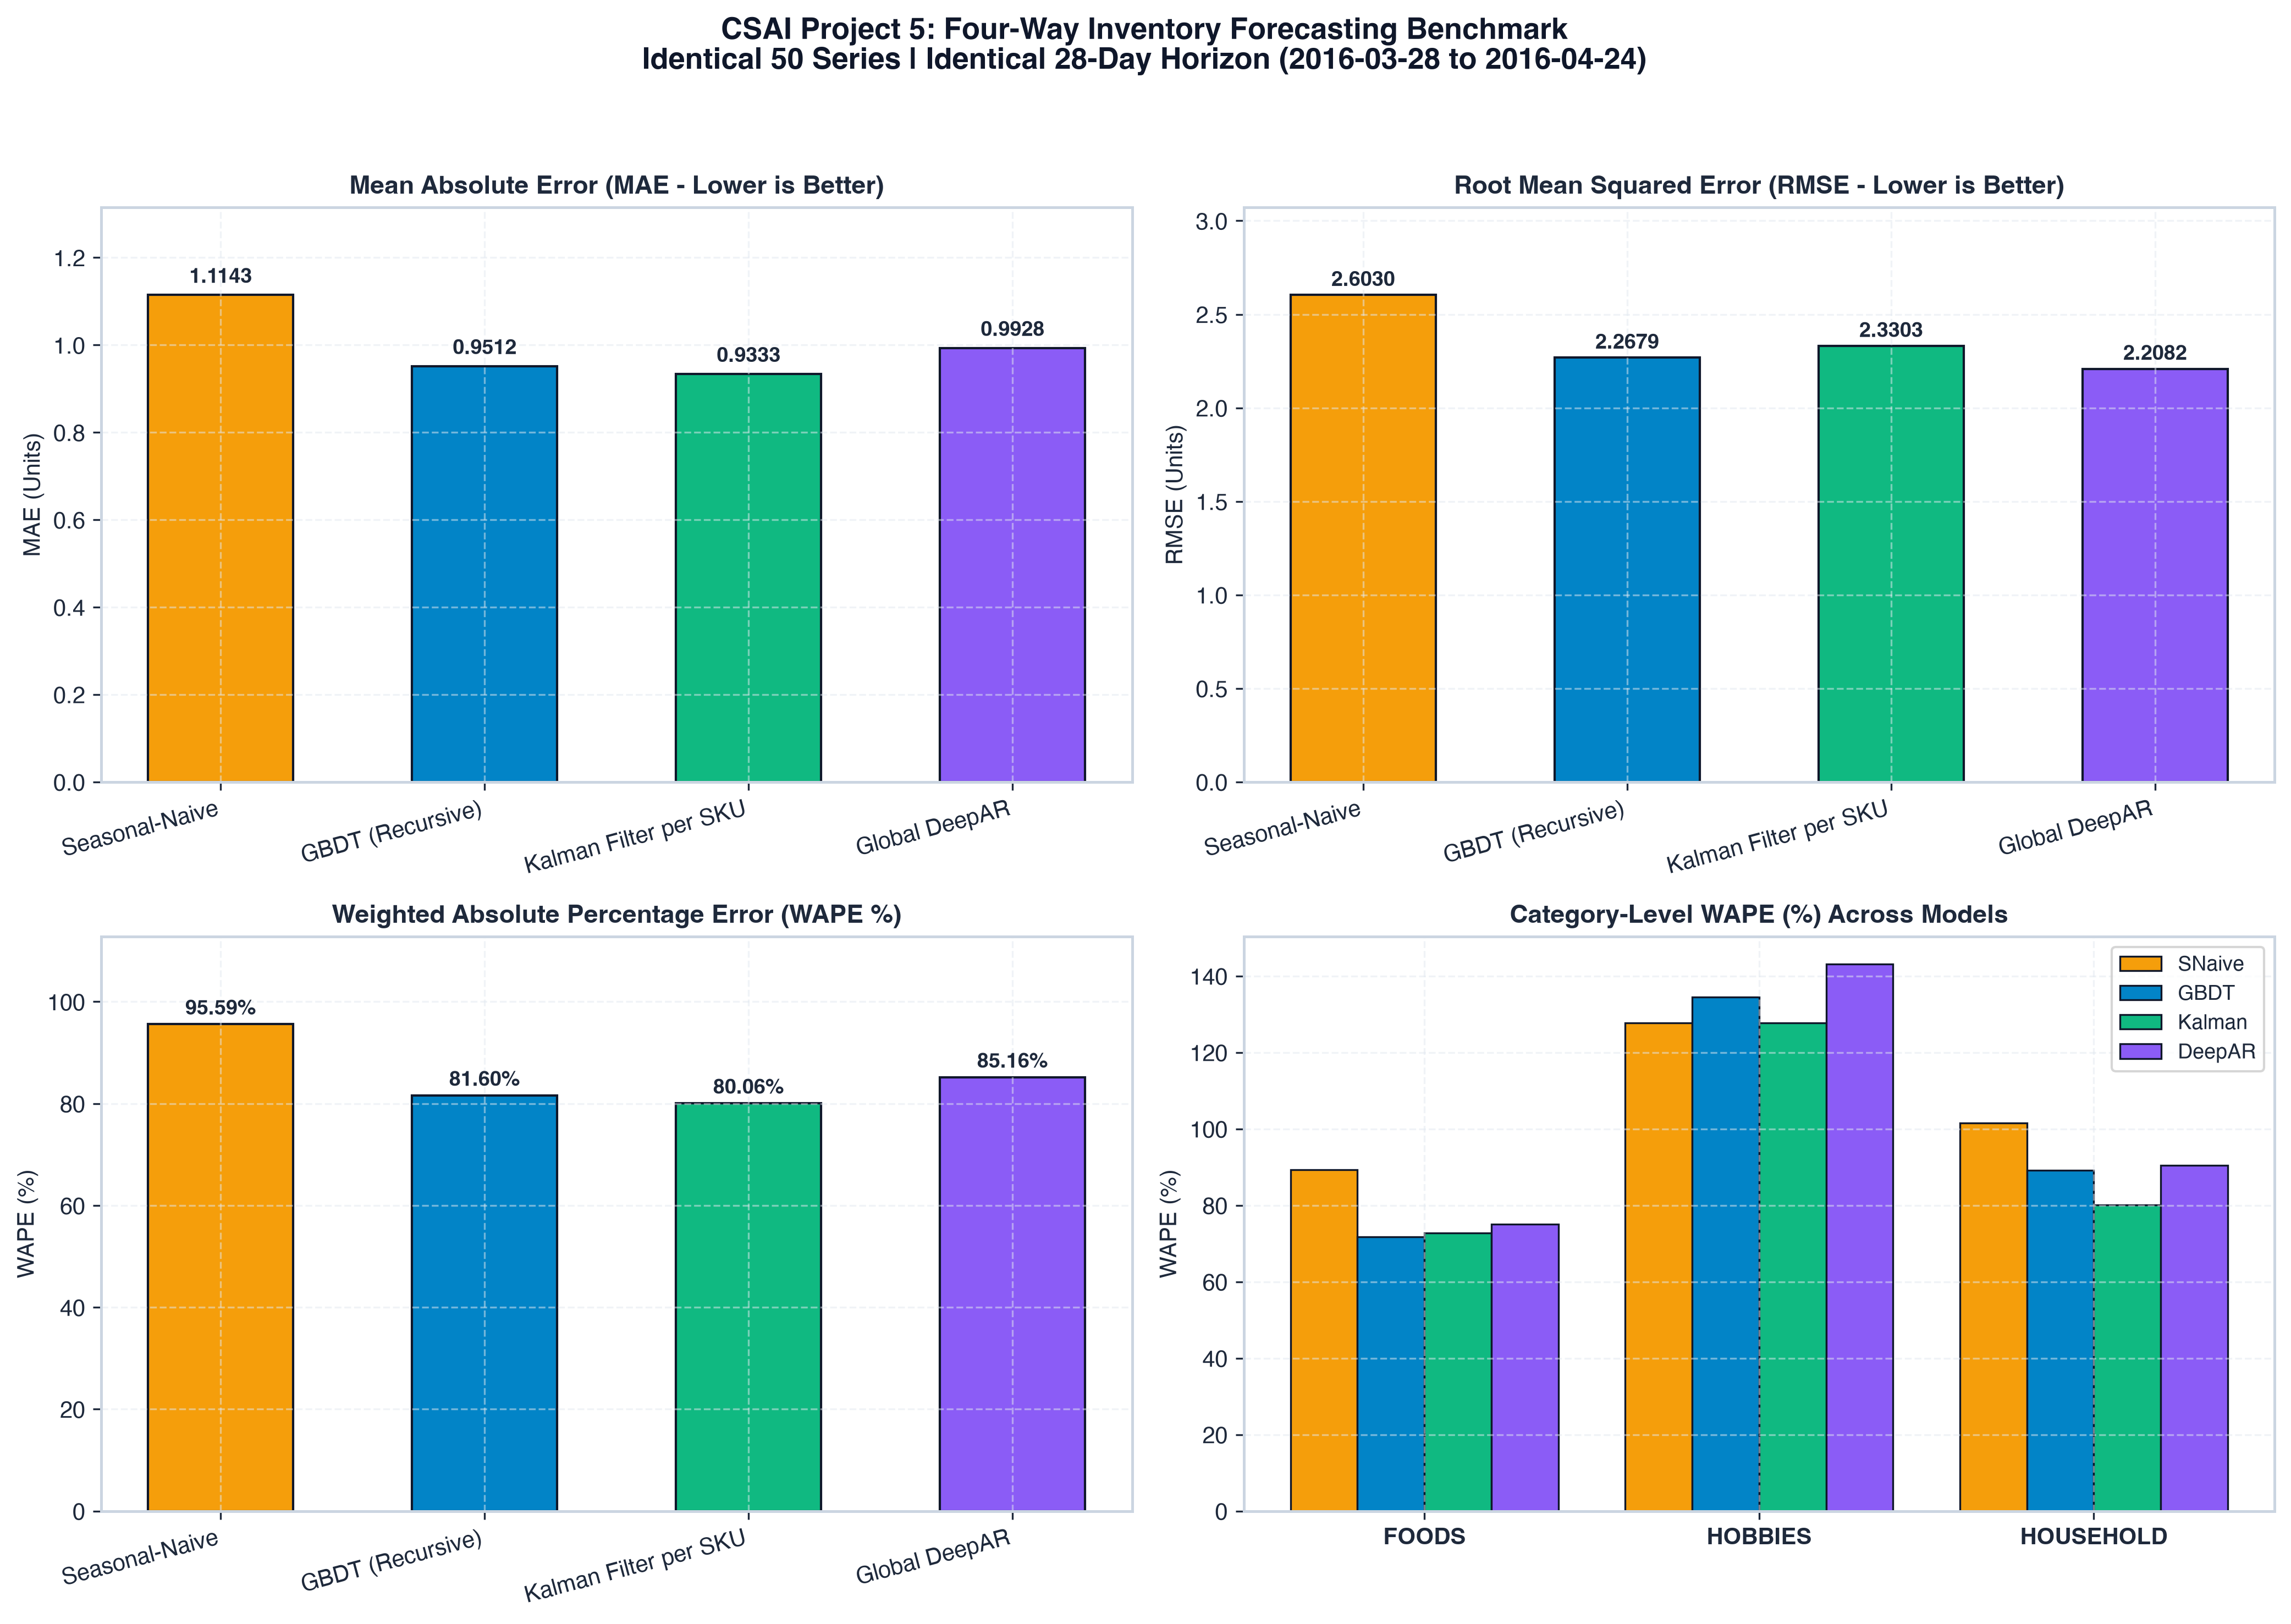
\includegraphics[width=\columnwidth]{16_four_way_model_comparison.png}
    \caption{Four-way model benchmark comparing MAE, RMSE, and WAPE across Seasonal-Naive, GBDT, Kalman Filter, and Global DeepAR.}
    \label{fig:four_way}
\end{figure}

\begin{figure}[htbp]
    \centering
    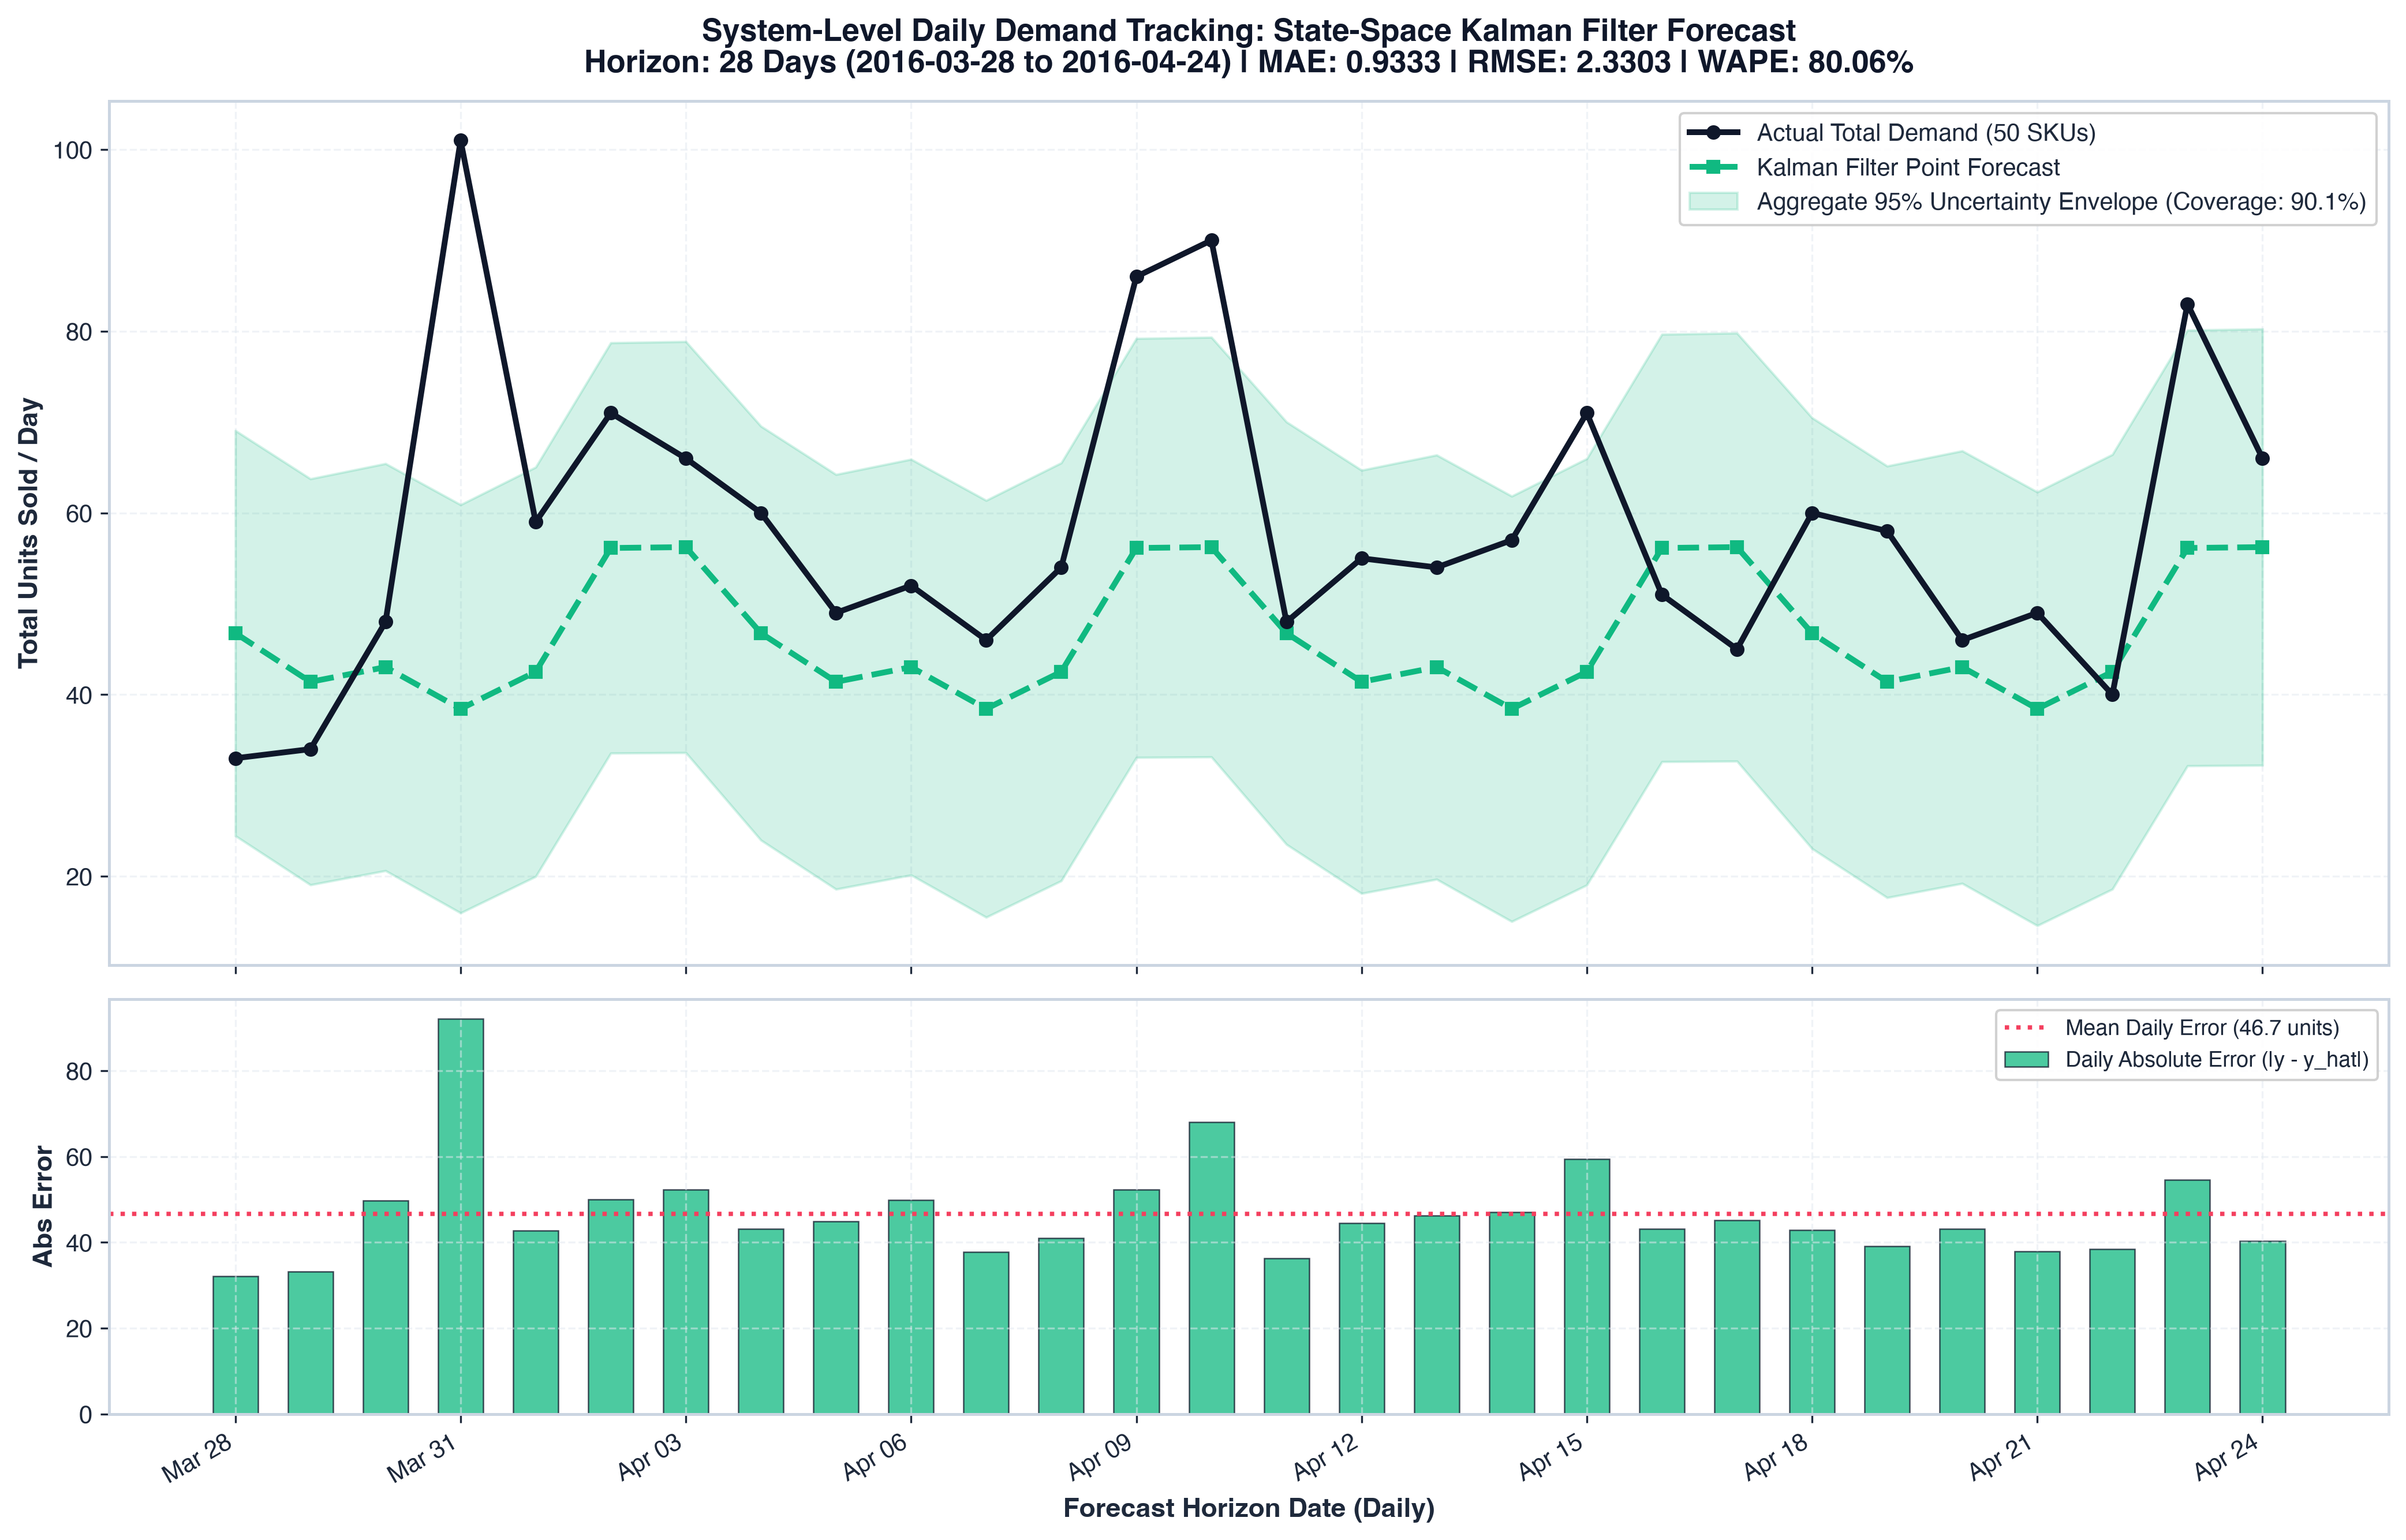
\includegraphics[width=\columnwidth]{13_kalman_aggregate_tracking.png}
    \caption{Kalman Filter aggregate tracking: system-level daily demand with 95\% prediction interval envelope.}
    \label{fig:kalman_tracking}
\end{figure}

\begin{figure}[htbp]
    \centering
    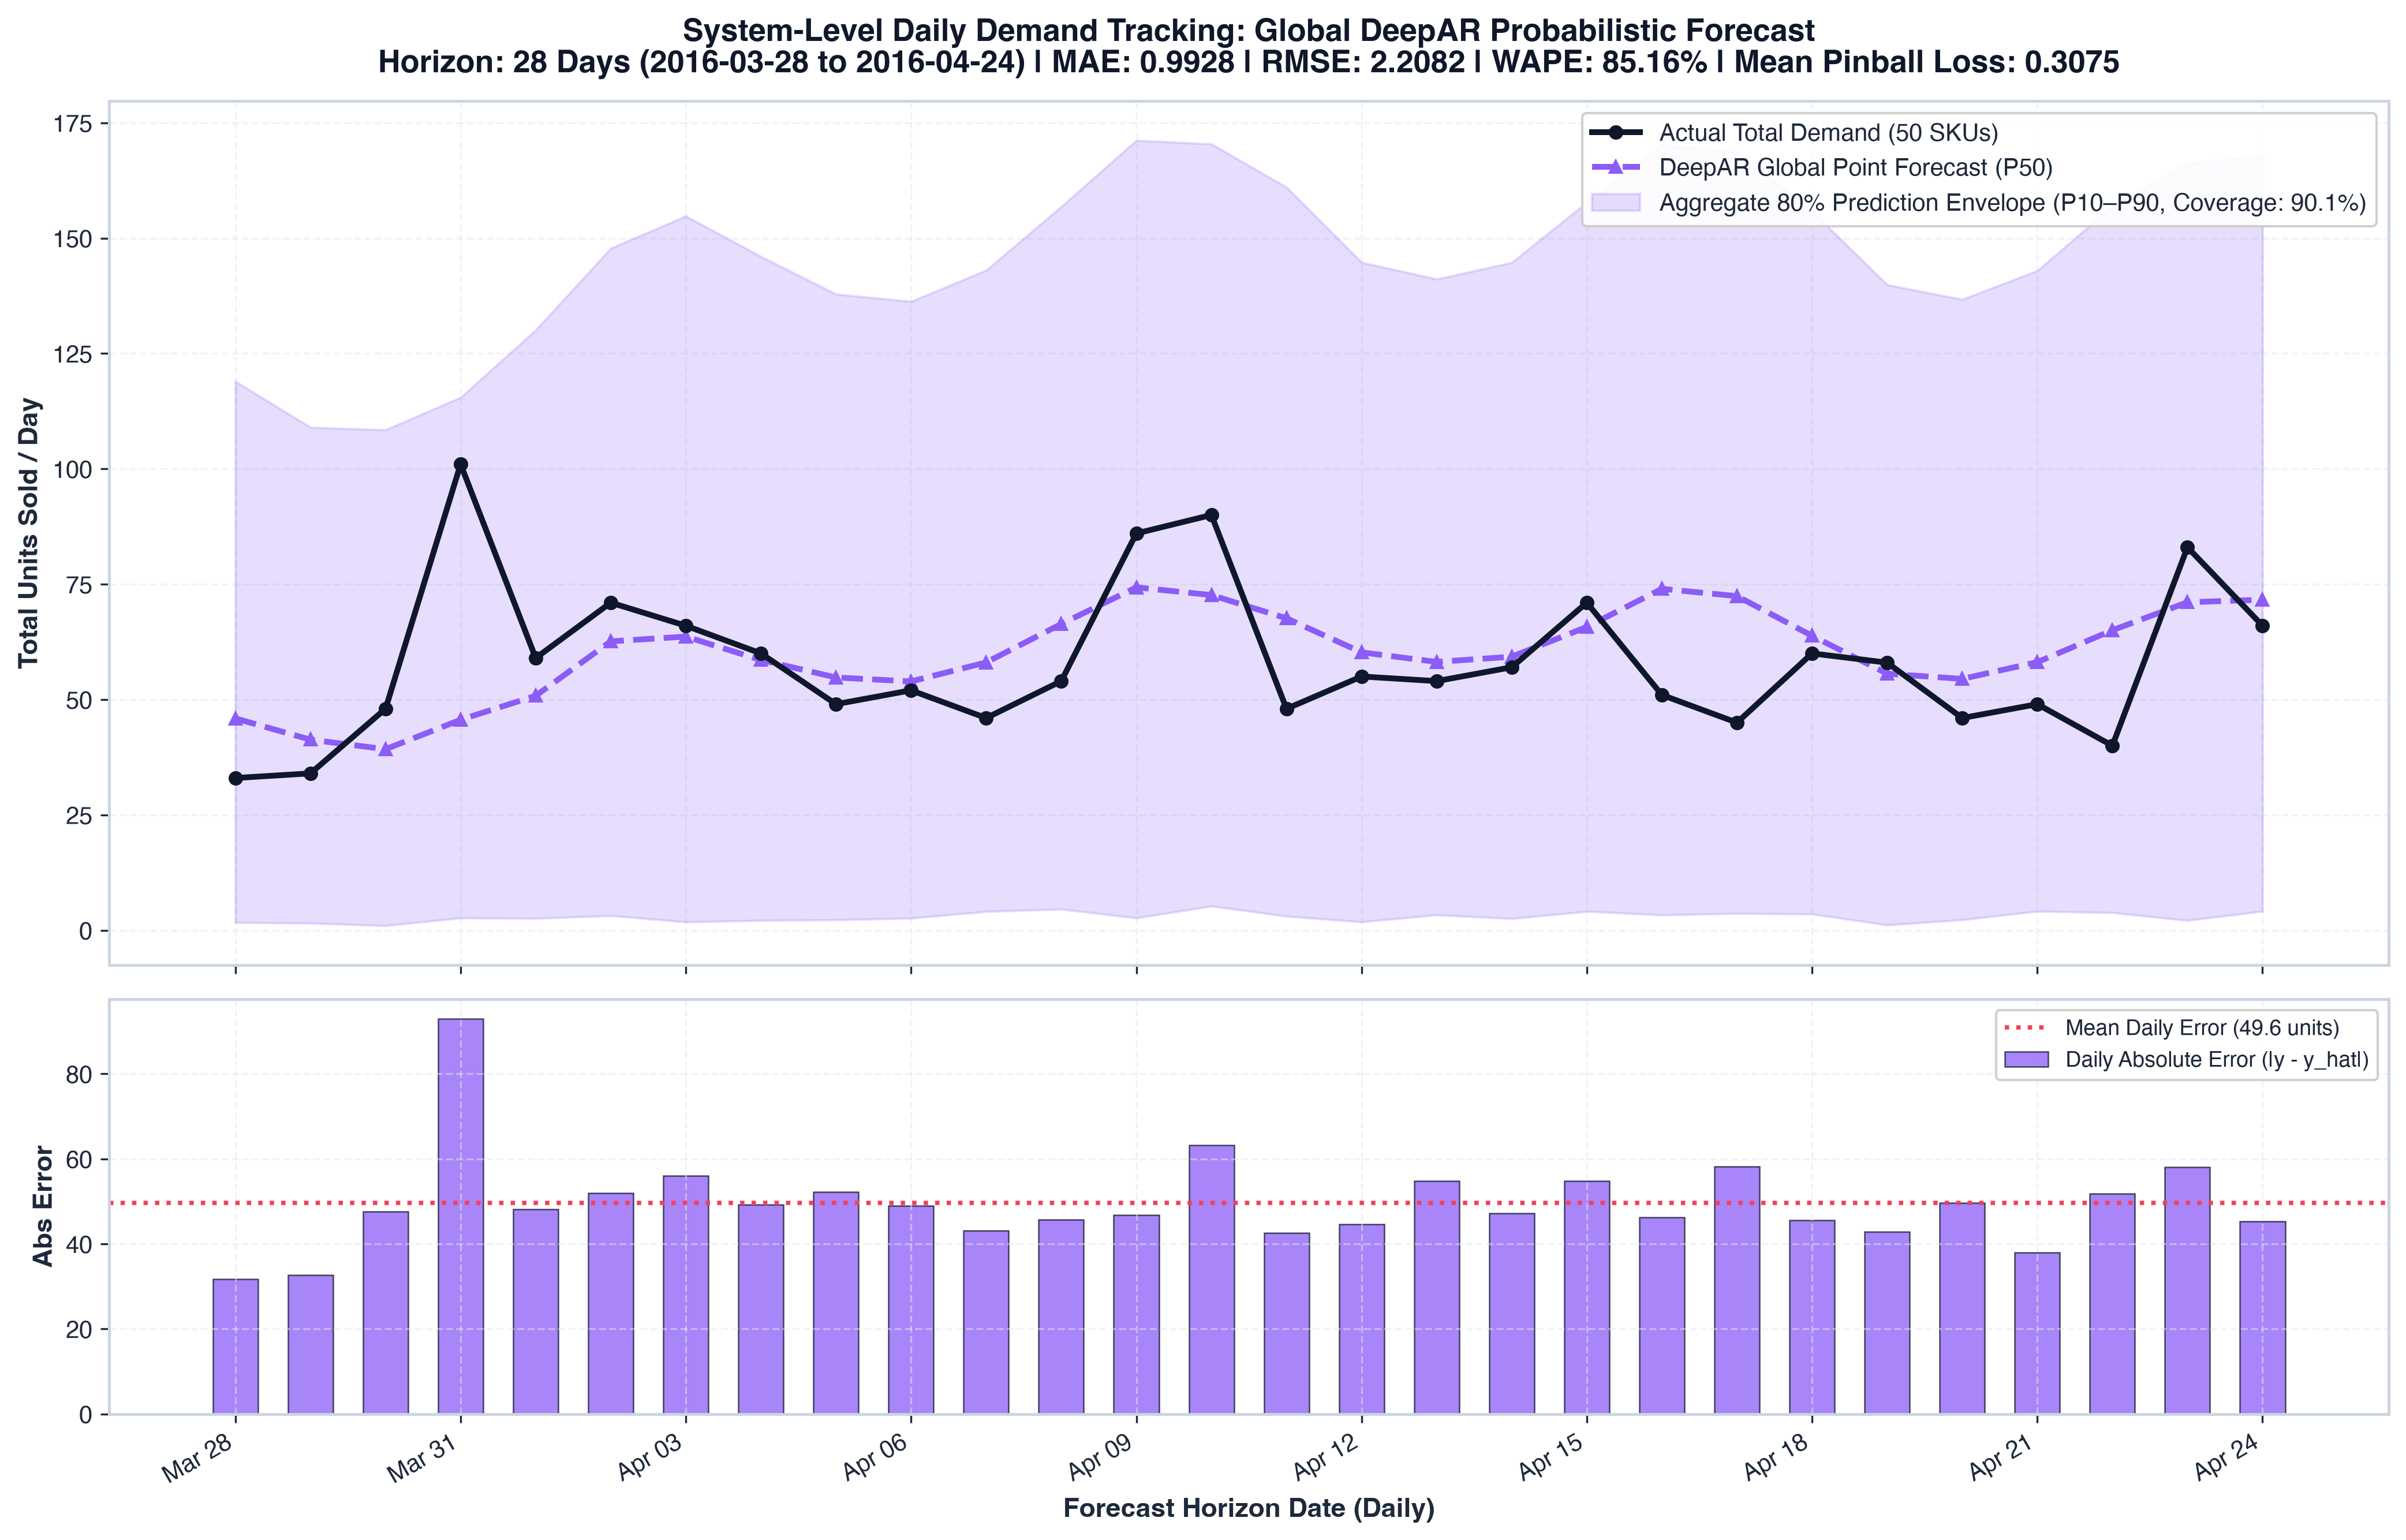
\includegraphics[width=\columnwidth]{deepar_forecasts.png}
    \caption{DeepAR system-level forecasts with 80\% prediction interval envelope showing aggregate demand tracking.}
    \label{fig:deepar_forecasts}
\end{figure}

\begin{figure}[htbp]
    \centering
    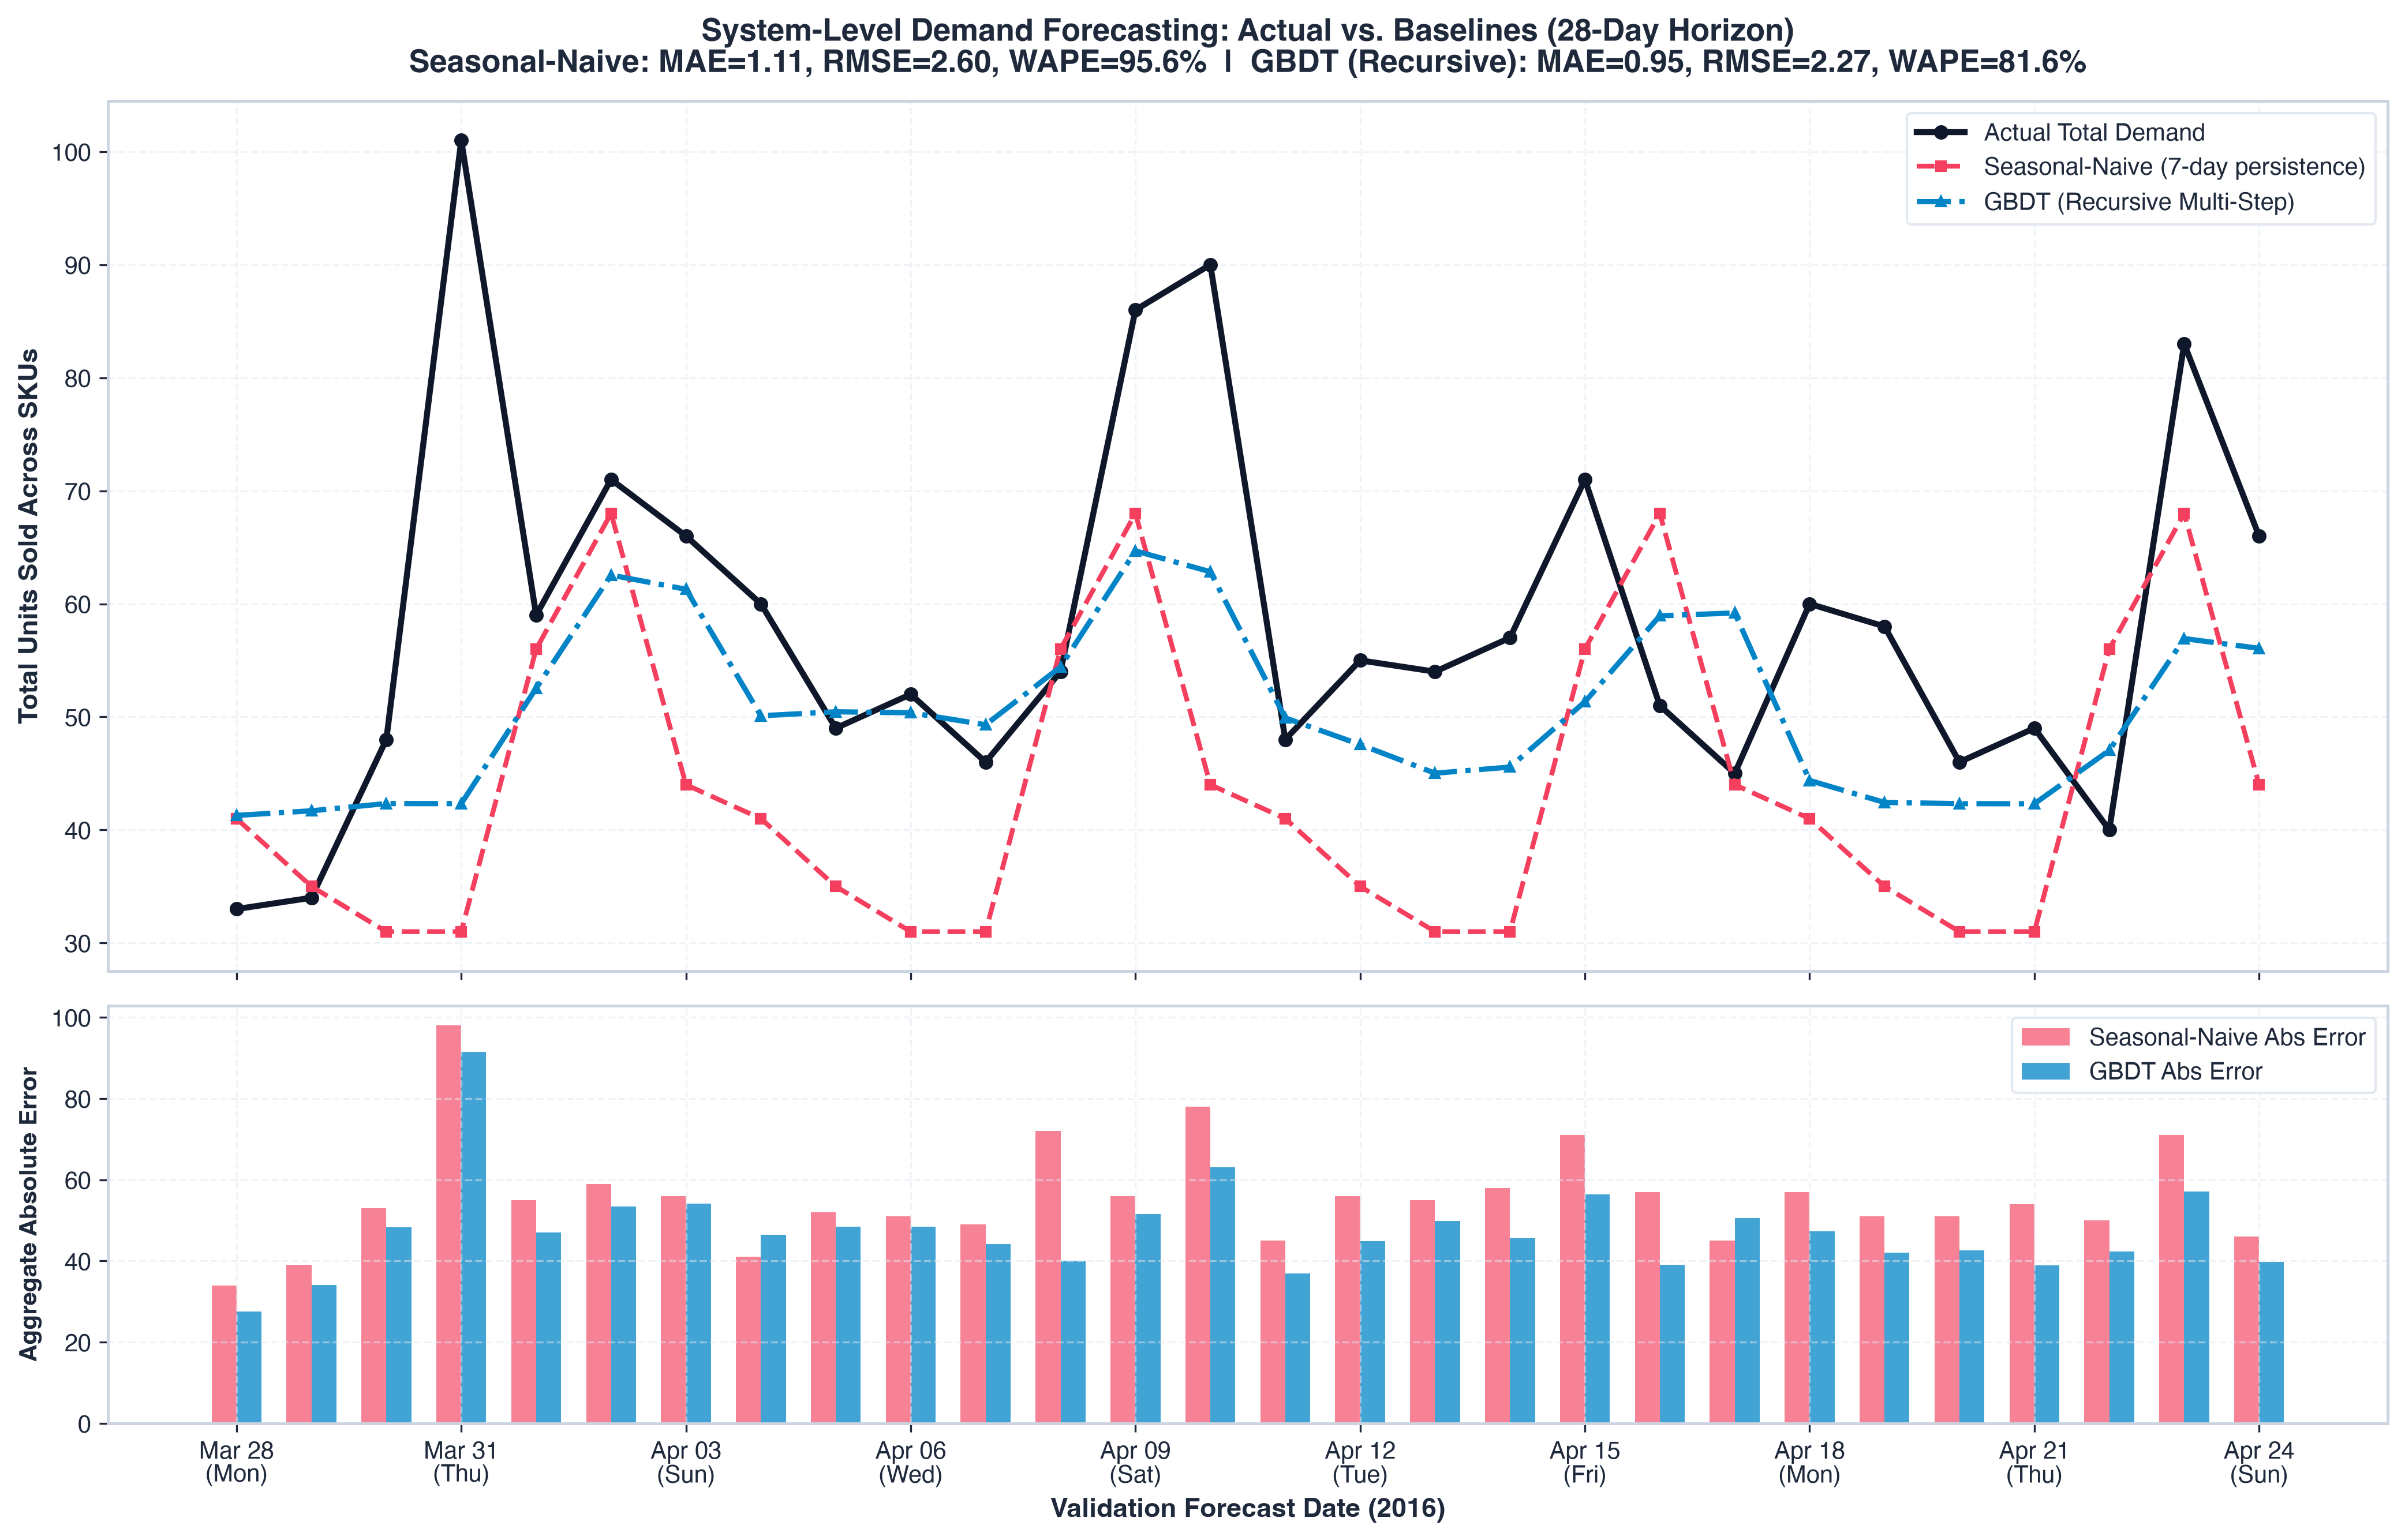
\includegraphics[width=\columnwidth]{10_baseline_aggregate_comparison.png}
    \caption{Baseline aggregate forecast comparison: 28-day daily system demand versus Seasonal-Naive and GBDT predictions.}
    \label{fig:baseline_comparison}
\end{figure}

% ══════════════════════════════════════════════════════════════════════════
% VII. DISCUSSION
% ══════════════════════════════════════════════════════════════════════════
\section{Discussion}

\subsection{Model Selection Trade-Offs}

The results demonstrate that model performance depends critically on the evaluation metric:

\begin{itemize}
    \item \textbf{Minimizing average absolute error (MAE/WAPE):} The Kalman Filter is the optimal choice. Its structural decomposition into local level and weekly seasonality enables rapid adaptation to individual SKU shifts without suffering from recursive variance dampening.

    \item \textbf{Minimizing large-error sensitivity (RMSE):} Global DeepAR is the preferred model. Its shared recurrent representation penalizes extreme deviations while generalizing across sparse series through cross-SKU statistical sharing.

    \item \textbf{Uncertainty quantification:} Both models provide principled prediction intervals, but through fundamentally different mechanisms---exact analytical covariance propagation (Kalman) versus empirical Monte Carlo quantile estimation (DeepAR).
\end{itemize}

\subsection{Architectural Comparison: Local vs.\ Global}

The Kalman Filter operates as 50 independent state-space models with zero cross-series sharing, relying purely on structural dynamics (level and seasonality). DeepAR trains a single unified network that shares representations across all SKUs via static entity embeddings, calendar cyclical signals, event markers, and SNAP schedules.

This fundamental architectural difference explains the performance divergence: the Kalman Filter excels at capturing local, SKU-specific level shifts and weekly patterns, while DeepAR benefits from cross-series regularization that dampens extreme prediction errors.

\subsection{Recursive Rollout Challenges}

Both the GBDT and DeepAR models face the challenge of compounding errors during recursive multi-step forecasting. As the horizon extends from Day 1 to Day 28, predicted values substituted into lag features can dampen variance or amplify errors. The Kalman Filter avoids this by maintaining an explicit state-space formulation with propagated uncertainty.

\subsection{Intermittent Demand Handling}

The predominance of intermittent and lumpy demand patterns (90.84\% of SKUs) validates the choice of state-space and probabilistic neural approaches over standard regression models. The Kalman Filter treats zero sales as legitimate observations of zero demand, preserving the intermittent signal structure. DeepAR handles this through scale normalization and non-negative clipping of Monte Carlo samples.

% ══════════════════════════════════════════════════════════════════════════
% VIII. LIMITATIONS
% ══════════════════════════════════════════════════════════════════════════
\section{Limitations}

Several limitations should be noted when interpreting the results:

\begin{enumerate}
    \item \textbf{Limited evaluation scope:} The evaluation covers 50 product-store series over a single 28-day horizon. Results may differ when evaluated across the full M5 dataset (30,490 series) or multiple rolling forecast origins.

    \item \textbf{Validation consistency:} The comparison should be interpreted only after confirming that all models use identical validation observations and consistent metric calculations, which has been ensured in this study.

    \item \textbf{DeepAR interval calibration:} While DeepAR achieves 91.79\% coverage at the 80\% nominal level, this over-coverage suggests potential for tighter intervals. A separate assessment of interval sharpness and calibration is warranted.

    \item \textbf{Hyperparameter sensitivity:} The DeepAR results are subject to training hyperparameter choices (learning rate, hidden dimension, number of epochs). A comprehensive hyperparameter search may yield different rankings.

    \item \textbf{Static Kalman parameters:} The Kalman Filter uses heuristic parameter estimation rather than maximum likelihood optimization. Adaptive or learned parameters could further improve performance.
\end{enumerate}

% ══════════════════════════════════════════════════════════════════════════
% IX. CONCLUSION
% ══════════════════════════════════════════════════════════════════════════
\section{Conclusion}

This paper presents a rigorous comparative study of four demand forecasting methodologies on the Walmart M5 dataset under strict zero-leakage evaluation conditions. The key conclusions are:

\begin{enumerate}
    \item The \textbf{Kalman Filter} is the strongest choice when minimizing average absolute and aggregate relative errors is the priority, achieving 16.25\% lower MAE and WAPE relative to the Seasonal-Naive baseline.

    \item \textbf{Global DeepAR} is a valuable alternative when larger errors and prediction uncertainty are important considerations, achieving the lowest RMSE (15.24\% reduction over baseline) and providing calibrated probabilistic prediction intervals.

    \item \textbf{GBDT (LightGBM)} provides a strong balance across all metrics with consistent 12--15\% improvements over the baseline, while being computationally efficient and interpretable through feature importance analysis.

    \item \textbf{No single model is best across every metric}, reinforcing that model selection in inventory forecasting must be aligned with the specific operational objective---whether minimizing average forecast error for routine replenishment, controlling worst-case errors for safety stock planning, or quantifying uncertainty for risk management.
\end{enumerate}

Future work should explore hybrid architectures that combine Kalman Filter state estimates as input features to the DeepAR global network, potentially capturing both local state dynamics and global cross-series patterns.

% ══════════════════════════════════════════════════════════════════════════
% REFERENCES
% ══════════════════════════════════════════════════════════════════════════
\begin{thebibliography}{10}

\bibitem{makridakis2022m5}
S.~Makridakis, E.~Spiliotis, and V.~Assimakopoulos,
``M5 accuracy competition: Results, findings, and conclusions,''
\textit{International Journal of Forecasting}, vol.~38, no.~4, pp.~1346--1364, 2022.

\bibitem{syntetos2005accuracy}
A.~A.~Syntetos, J.~E.~Boylan, and J.~D.~Croston,
``On the categorization of demand patterns,''
\textit{Journal of the Operational Research Society}, vol.~56, no.~5, pp.~495--503, 2005.

\bibitem{ke2017lightgbm}
G.~Ke, Q.~Meng, T.~Finley, T.~Wang, W.~Chen, W.~Ma, Q.~Ye, and T.-Y.~Liu,
``LightGBM: A highly efficient gradient boosting decision tree,''
in \textit{Advances in Neural Information Processing Systems~30}, 2017, pp.~3146--3154.

\bibitem{salinas2020deepar}
D.~Salinas, V.~Flunkert, J.~Gasthaus, and T.~Januschowski,
``DeepAR: Probabilistic forecasting with autoregressive recurrent networks,''
\textit{International Journal of Forecasting}, vol.~36, no.~3, pp.~1181--1191, 2020.

\bibitem{kalman1960new}
R.~E.~Kalman,
``A new approach to linear filtering and prediction problems,''
\textit{Journal of Basic Engineering}, vol.~82, no.~1, pp.~35--45, 1960.

\bibitem{harvey1990forecasting}
A.~C.~Harvey,
\textit{Forecasting, Structural Time Series Models and the Kalman Filter}.
Cambridge University Press, 1990.

\bibitem{durbin2012time}
J.~Durbin and S.~J.~Koopman,
\textit{Time Series Analysis by State Space Methods}, 2nd~ed.
Oxford University Press, 2012.

\bibitem{hochreiter1997long}
S.~Hochreiter and J.~Schmidhuber,
``Long short-term memory,''
\textit{Neural Computation}, vol.~9, no.~8, pp.~1735--1780, 1997.

\bibitem{hyndman2018forecasting}
R.~J.~Hyndman and G.~Athanasopoulos,
\textit{Forecasting: Principles and Practice}, 2nd~ed.
OTexts, Melbourne, Australia, 2018.
[Online]. Available: \url{https://otexts.com/fpp2/}

\bibitem{benidis2022deep}
K.~Benidis, S.~S.~Rangapuram, V.~Flunkert, Y.~Wang, D.~Maddix, C.~Turkmen, J.~Gasthaus, M.~Bohlke-Schneider, D.~Salinas, L.~Stella, F.~X.~Aubet, L.~Callot, and T.~Januschowski,
``Deep learning for time series forecasting: Tutorial and literature survey,''
\textit{ACM Computing Surveys}, vol.~55, no.~6, pp.~1--36, 2022.

\end{thebibliography}

\end{document}
